%!TEX TS-program = xelatex
\documentclass[a4paper,14pt]{article}


%%% Работа с русским языком
\usepackage[english,russian]{babel}   %% загружает пакет многоязыковой вёрстки
\usepackage{fontspec}      %% подготавливает загрузку шрифтов Open Type, True Type и др.
\defaultfontfeatures{Ligatures={TeX},Renderer=Basic}  %% свойства шрифтов по умолчанию
\setmainfont[Ligatures={TeX,Historic}]{Times New Roman} %% задаёт основной шрифт документа
\setsansfont{Comic Sans MS}                    %% задаёт шрифт без засечек
\setmonofont{Courier New}
\usepackage{indentfirst}
\frenchspacing

\renewcommand{\epsilon}{\ensuremath{\varepsilon}}
\renewcommand{\phi}{\ensuremath{\varphi}}
\renewcommand{\kappa}{\ensuremath{\varkappa}}
\renewcommand{\le}{\ensuremath{\leqslant}}
\renewcommand{\leq}{\ensuremath{\leqslant}}
\renewcommand{\ge}{\ensuremath{\geqslant}}
\renewcommand{\geq}{\ensuremath{\geqslant}}
\renewcommand{\emptyset}{\varnothing}

%%% Дополнительная работа с математикой
\usepackage{amsmath,amsfonts,amssymb,amsthm,mathtools} % AMS
\usepackage{icomma} % "Умная" запятая: $0,2$ --- число, $0, 2$ --- перечисление

%% Номера формул
%\mathtoolsset{showonlyrefs=true} % Показывать номера только у тех формул, на которые есть \eqref{} в тексте.
%\usepackage{leqno} % Нумерация формул слева	

%% Перенос знаков в формулах (по Львовскому)
\newcommand*{\hm}[1]{#1\nobreak\discretionary{}
	{\hbox{$\mathsurround=0pt #1$}}{}}

%%% Работа с картинками
\usepackage{graphicx}  % Для вставки рисунков
\graphicspath{{images/}}  % папки с картинками
\setlength\fboxsep{3pt} % Отступ рамки \fbox{} от рисунка
\setlength\fboxrule{1pt} % Толщина линий рамки \fbox{}
\usepackage{wrapfig} % Обтекание рисунков текстом

%%% Работа с таблицами
\usepackage{array,tabularx,tabulary,booktabs} % Дополнительная работа с таблицами
\usepackage{longtable}  % Длинные таблицы
\usepackage{multirow} % Слияние строк в таблице
\usepackage{float}% http://ctan.org/pkg/float

%%% Программирование
\usepackage{etoolbox} % логические операторы


%%% Страница
\usepackage{extsizes} % Возможность сделать 14-й шрифт
\usepackage{geometry} % Простой способ задавать поля
\geometry{top=20mm}
\geometry{bottom=20mm}
\geometry{left=20mm}
\geometry{right=10mm}
%
%\usepackage{fancyhdr} % Колонтитулы
% 	\pagestyle{fancy}
%\renewcommand{\headrulewidth}{0pt}  % Толщина линейки, отчеркивающей верхний колонтитул
% 	\lfoot{Нижний левый}
% 	\rfoot{Нижний правый}
% 	\rhead{Верхний правый}
% 	\chead{Верхний в центре}
% 	\lhead{Верхний левый}
%	\cfoot{Нижний в центре} % По умолчанию здесь номер страницы

\usepackage{setspace} % Интерлиньяж
\onehalfspacing % Интерлиньяж 1.5
%\doublespacing % Интерлиньяж 2
%\singlespacing % Интерлиньяж 1

\usepackage{lastpage} % Узнать, сколько всего страниц в документе.

\usepackage{soul} % Модификаторы начертания

\usepackage{hyperref}
\usepackage[usenames,dvipsnames,svgnames,table,rgb]{xcolor}
\hypersetup{				% Гиперссылки
	unicode=true,           % русские буквы в раздела PDF
	pdftitle={Разработка программной системы для автоматической генерации графа диалогов по текстам пьес.},   % Заголовок
	pdfauthor={Подчезерцев А.Е.},      % Автор
	pdfsubject={ВКР},      % Тема
	pdfcreator={Подчезерцев А.Е.}, % Создатель
	pdfproducer={Подчезерцев А.Е.}, % Производитель
	pdfkeywords={keyword1} {key2} {key3}, % Ключевые слова
	colorlinks=true,       	% false: ссылки в рамках; true: цветные ссылки
	linkcolor=black,          % внутренние ссылки
	citecolor=black,        % на библиографию
	filecolor=magenta,      % на файлы
	urlcolor=black           % на URL
}
\makeatletter 
\def\@biblabel#1{#1. } 
\makeatother
\usepackage{cite} % Работа с библиографией
%\usepackage[superscript]{cite} % Ссылки в верхних индексах
%\usepackage[nocompress]{cite} % 
\usepackage{csquotes} % Еще инструменты для ссылок

\usepackage{multicol} % Несколько колонок

\usepackage{tikz} % Работа с графикой
\usepackage{pgfplots}
\usepackage{pgfplotstable}

\usepackage{ dsfont }

\newcommand{\imref}[1]{рис.~\ref{#1}}

\usepackage{spreadtab}
\newcolumntype{K}[1]{@{}>{\centering\arraybackslash}p{#1cm}@{}}


\usepackage{xparse}
\usepackage{fancyvrb}

\RecustomVerbatimCommand{\VerbatimInput}{VerbatimInput}
{
	fontsize=\footnotesize    
}

\newcolumntype{?}[1]{!{\vrule width #1}}

\usepackage{tocloft}
\renewcommand{\cftsecleader}{\cftdotfill{\cftdotsep}}

\usepackage{pdfpages}

\usepackage{rotating}

\usepackage{pdflscape}

\usepackage{ragged2e}
\usepackage{microtype}

% Выравнивание по ширине без переносов слов
\justifying
\sloppy
\tolerance=500
\hyphenpenalty=10000
\emergencystretch=3em

% Подогнать таблицу под ширину страницы
\usepackage{adjustbox}

\usepackage{titlesec}

% ГОСТ заголовки таблицы
\usepackage[font=small]{caption}

\captionsetup[figure]{justification=centering,labelsep=period} % Картинки по центру, с точкой после рис

\DeclareCaptionLabelFormat{rightline}{\rightline{\bothIfFirst{#1}{ }#2}}
\captionsetup[table]{justification=centering,labelformat=rightline,labelsep=newline}

\newcommand{\tablecaption}[1]{\addtocounter{table}{1}\small \begin{flushright}\tablename \ \thetable\end{flushright}%	
	\begin{center}#1\end{center}}

\usepackage{enumerate}
\begin{document} 	
	
	\addcontentsline{toc}{section}{Приложение А}

\begin{flushright}
	Приложение А
\end{flushright}


\begin{center}
	Пример визуализации функции позиционного кодирования
\end{center}


\begin{figure}[H]
	\centering
	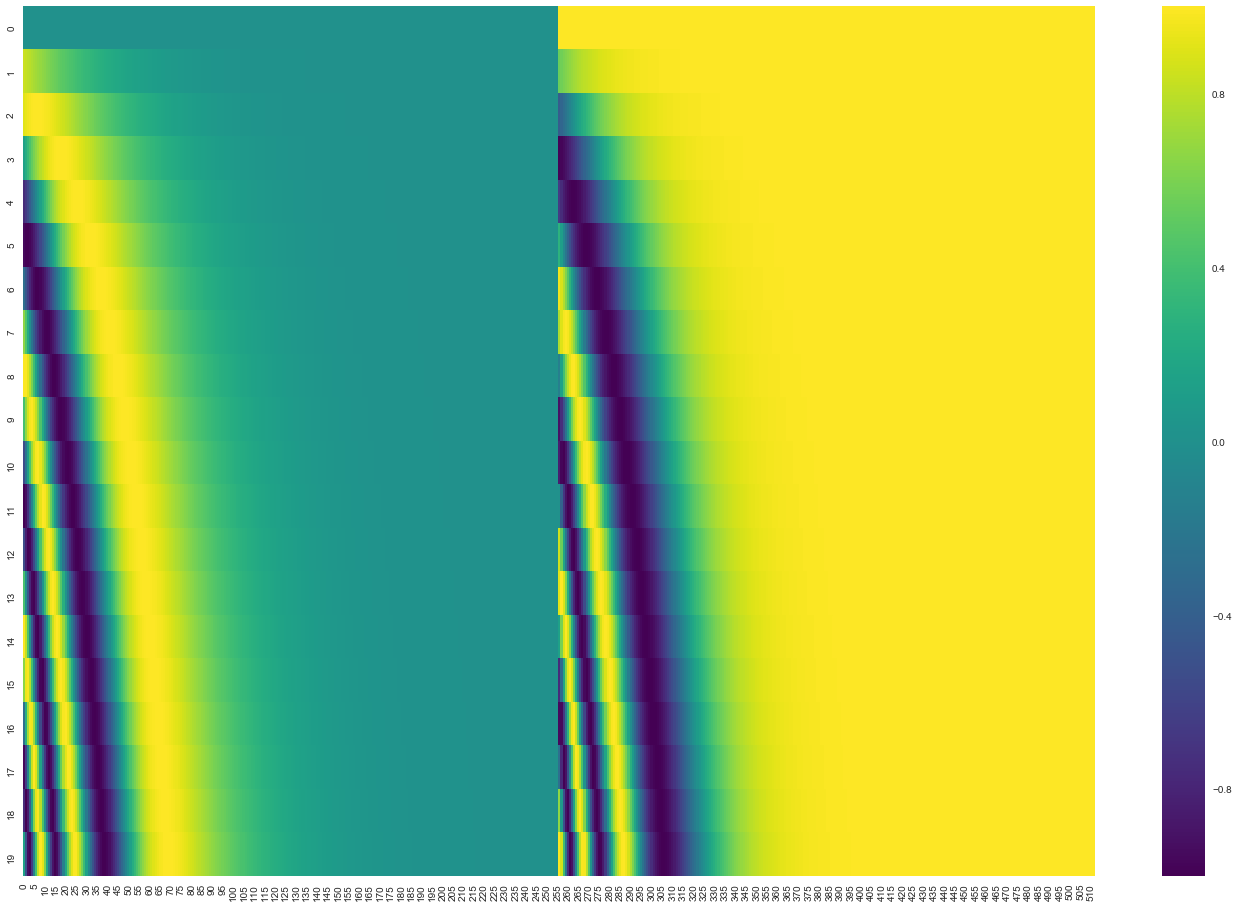
\includegraphics[width=0.95\linewidth]{image/v9dvohtljexbjop_vrykyyqdzbk}
	\caption*{Рис. А1. Пример визуализации функции позиционного кодирования}
	\label{fig:v9dvohtljexbjopvrykyyqdzbk}
\end{figure}

\newpage

\addcontentsline{toc}{section}{Приложение Б}

\begin{flushright}
	Приложение Б
\end{flushright}

\begin{center}
	Ссылки на исходные коды
\end{center}

Ссылка на github репозиторий \href{https://github.com/andrsolo21/hse_Af_Tr_BERT}{https://github.com/andrsolo21/hse\_Af\_Tr\_BERT}.

Ссылка на ноутбук с примером работы модели BERT: \href{https://github.com/andrsolo21/hse_Af_Tr_BERT/blob/main/new_hse_BERT_0.ipynb}{new\_hse\_BERT\_0.ipynb}.

Ссылка на ноутбук с примером работы модели ELMo:  \href{https://github.com/andrsolo21/hse_Af_Tr_BERT/blob/main/new_hse_ELMO_0.ipynb}{new\_hse\_ELMO\_0.ipynb}.

Ссылка на ноутбук с агрегацией результатов: \href{https://github.com/andrsolo21/hse_Af_Tr_BERT/blob/main/Visualization.ipynb}{Visualization.ipynb}.

\newpage

\addcontentsline{toc}{section}{Приложение В}

\begin{flushright}
	Приложение В
\end{flushright}

\begin{center}
	Визуализация эмбеддингов
\end{center}


\begin{figure}[H]
	\centering
	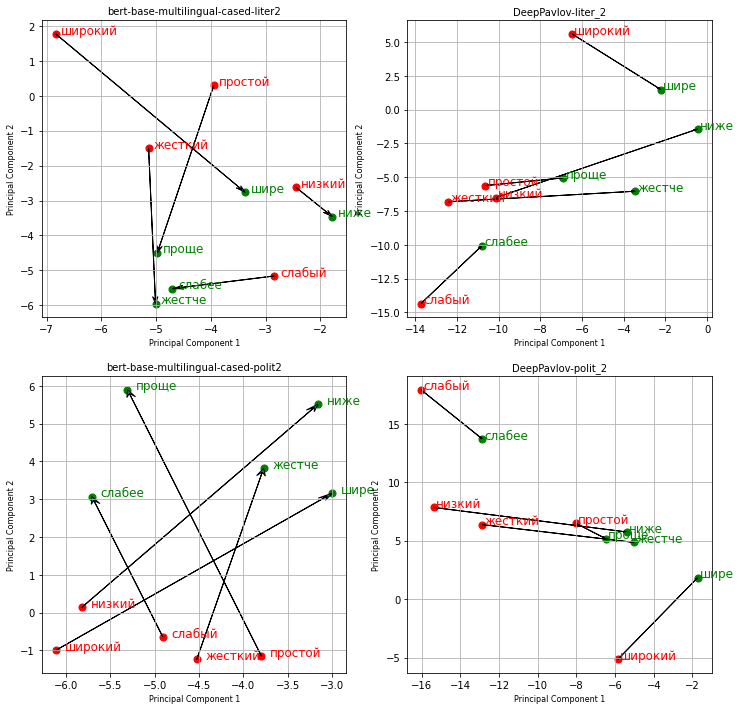
\includegraphics[width=0.95\linewidth]{image/pril_2}
	\caption*{Рис. В1. Визуализация эмбеддингов из группы <<прилагательное -- сравнительная степень>> для модели BERT с обработкой N-грамм через вычисление среднего эмбеддинга; Слева модель bert-base-multilingual-cased, справа от DeepPavlov; Верхние модели обучены на жанре литературы, нижние на политике}
	\label{fig:pril22}
\end{figure}

\begin{figure}[H]
	\centering
	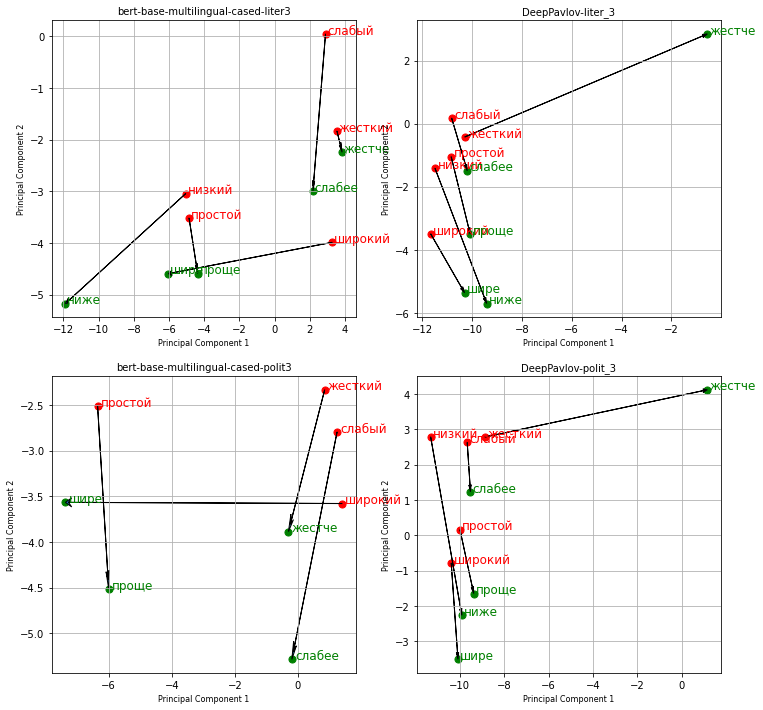
\includegraphics[width=0.95\linewidth]{image/pril_3}
	\caption*{Рис. В2. Визуализация эмбеддингов из группы <<прилагательное -- сравнительная степень>> для модели BERT с обработкой N-грамм через вычисление суммы эмбеддингов; Слева модель bert-base-multilingual-cased, справа от DeepPavlov; Верхние модели обучены на жанре литературы, нижние на политике}
	\label{fig:pril32}
\end{figure}

\begin{figure}[H]
	\centering
	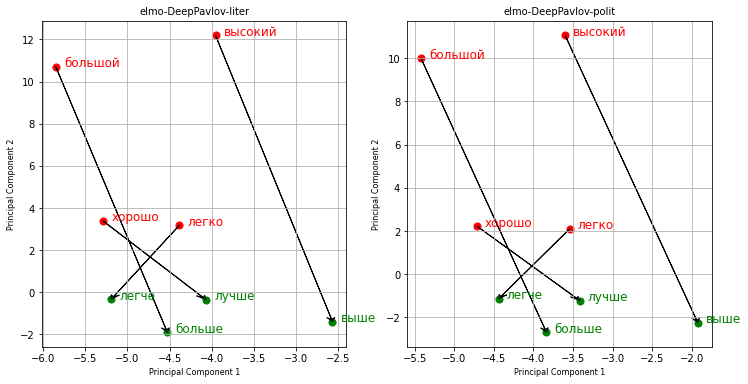
\includegraphics[width=0.95\linewidth]{image/elmo_pil}
	\caption*{Рис. В3. Визуализация эмбеддингов из группы <<прилагательное -- сравнительная степень>> для модели ELMo; Слева модель обучена на жанре литературы, справа на политике}
	\label{fig:elmopil2}
\end{figure}

\begin{figure}[H]
	\centering
	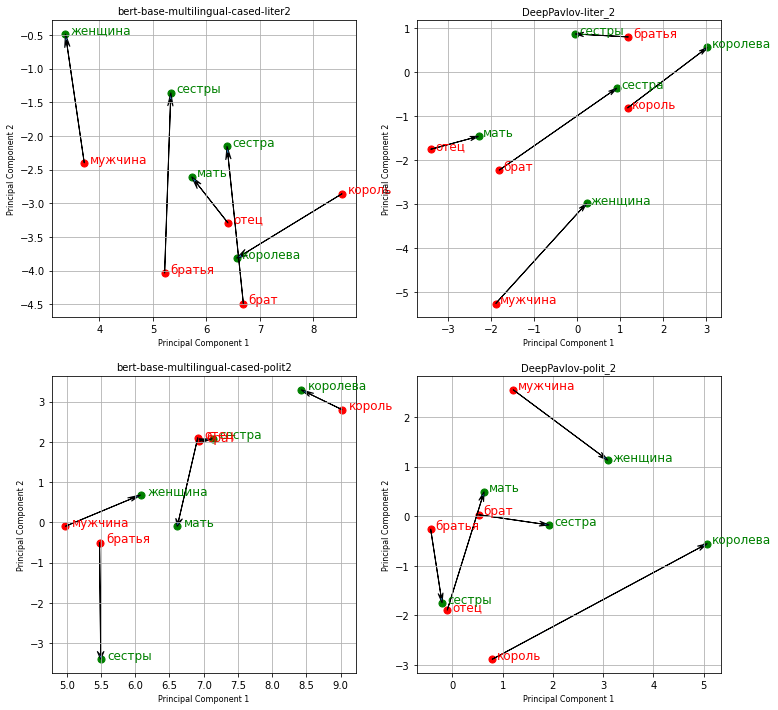
\includegraphics[width=0.95\linewidth]{image/fam_2}
	\caption*{Рис. В4. Визуализация эмбеддингов из группы <<мужской пол -- женский пол>> для модели BERT с обработкой N-грамм через вычисление среднего эмбеддинга; Слева модель bert-base-multilingual-cased, справа от DeepPavlov; Верхние модели обучены на жанре литературы, нижние на политике}
	\label{fig:fam2}
\end{figure}

\begin{figure}[H]
	\centering
	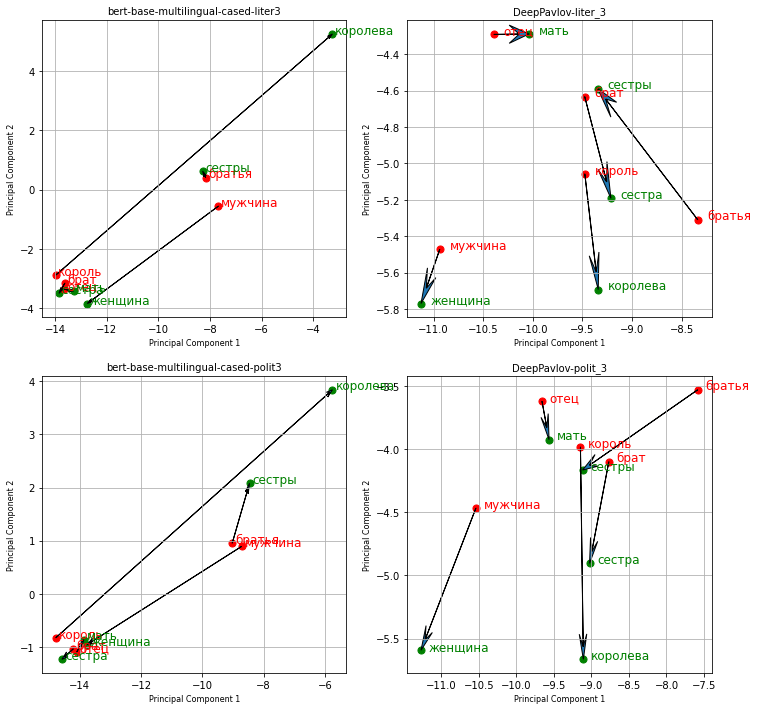
\includegraphics[width=0.95\linewidth]{image/fam_3}
	\caption*{Рис. В5. Визуализация эмбеддингов из группы <<мужской пол -- женский пол>> для модели BERT с обработкой N-грамм через вычисление суммы эмбеддингов; Слева модель bert-base-multilingual-cased, справа от DeepPavlov; Верхние модели обучены на жанре литературы, нижние на политике}
	\label{fig:fam3}
\end{figure}

\newpage

\addcontentsline{toc}{section}{Приложение Г}

\begin{flushright}
	Приложение Г
\end{flushright}

\begin{center}
	 Результаты тестирования моделей
\end{center}

\begin{figure}[H]
	\centering
	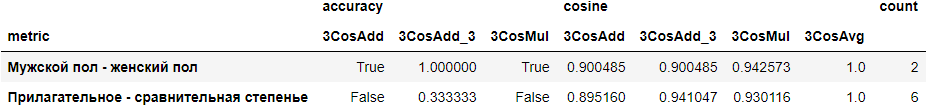
\includegraphics[width=0.9\linewidth]{image/res_bert-base-multilingual-cased-liter }
	\caption*{Рис. Г1. Результаты тестирования для модели bert-base-multilingual-cased-liter }
	\label{fig:resbert-base-multilingual-cased-liter }
\end{figure}

\begin{figure}[H]
	\centering
	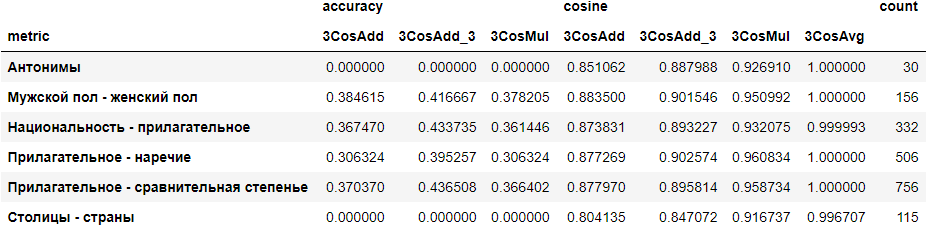
\includegraphics[width=0.9\linewidth]{image/res_bert-base-multilingual-cased-liter2 }
	\caption*{Рис. Г2. Результаты тестирования для модели bert-base-multilingual-cased-liter2 }
	\label{fig:resbert-base-multilingual-cased-liter2 }
\end{figure}

\begin{figure}[H]
	\centering
	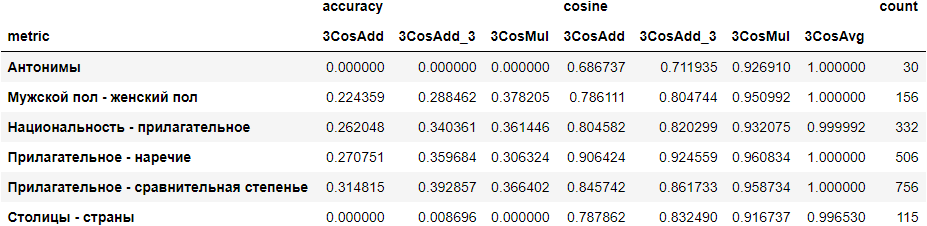
\includegraphics[width=0.9\linewidth]{image/res_bert-base-multilingual-cased-liter3 }
	\caption*{Рис. Г3. Результаты тестирования для модели bert-base-multilingual-cased-liter3 }
	\label{fig:resbert-base-multilingual-cased-liter3 }
\end{figure}

\begin{figure}[H]
	\centering
	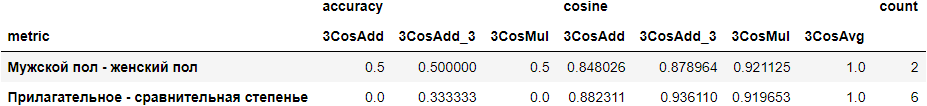
\includegraphics[width=0.9\linewidth]{image/res_bert-base-multilingual-cased-polit }
	\caption*{Рис. Г4. Результаты тестирования для модели bert-base-multilingual-cased-polit }
	\label{fig:resbert-base-multilingual-cased-polit }
\end{figure}

\begin{figure}[H]
	\centering
	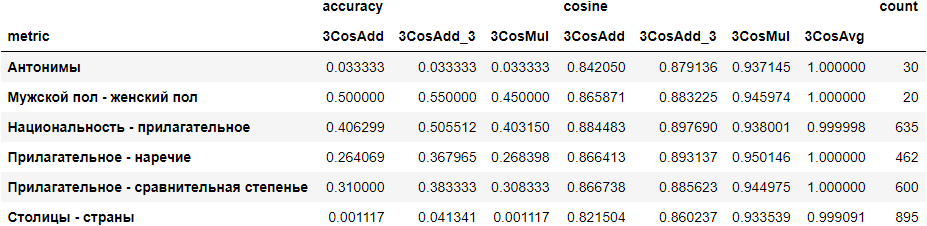
\includegraphics[width=0.9\linewidth]{image/res_bert-base-multilingual-cased-polit2 }
	\caption*{Рис. Г5. Результаты тестирования для модели bert-base-multilingual-cased-polit2 }
	\label{fig:resbert-base-multilingual-cased-polit2 }
\end{figure}

\begin{figure}[H]
	\centering
	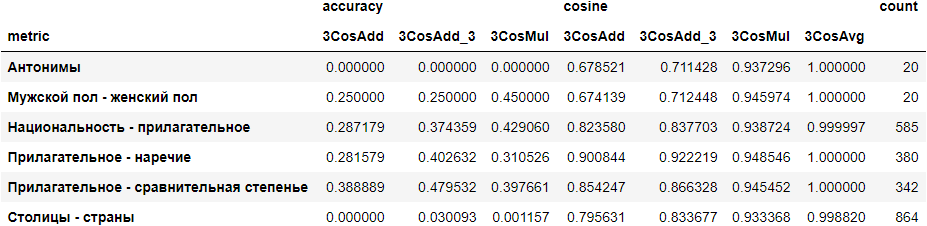
\includegraphics[width=0.9\linewidth]{image/res_bert-base-multilingual-cased-polit3 }
	\caption*{Рис. Г6. Результаты тестирования для модели bert-base-multilingual-cased-polit3 }
	\label{fig:resbert-base-multilingual-cased-polit3 }
\end{figure}

\begin{figure}[H]
	\centering
	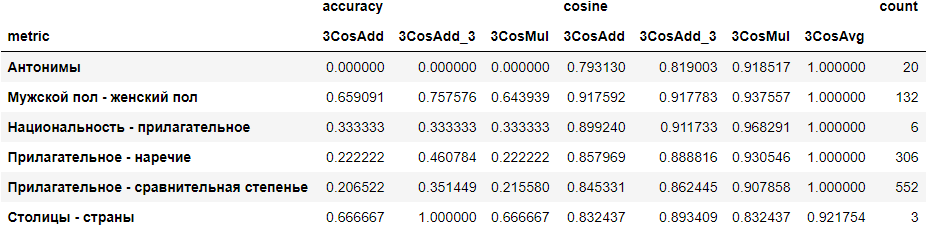
\includegraphics[width=0.9\linewidth]{image/res_DeepPavlov-liter }
	\caption*{Рис. Г7. Результаты тестирования для модели DeepPavlov-liter }
	\label{fig:resDeepPavlov-liter }
\end{figure}

\begin{figure}[H]
	\centering
	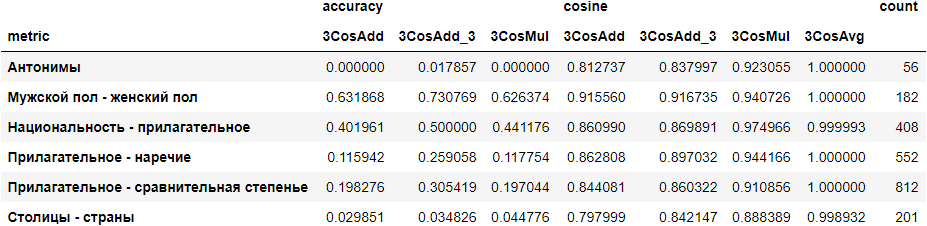
\includegraphics[width=0.9\linewidth]{image/res_DeepPavlov-liter_2 }
	\caption*{Рис. Г8. Результаты тестирования для модели DeepPavlov-liter\_2 }
	\label{fig:resDeepPavlov-liter2 }
\end{figure}

\begin{figure}[H]
	\centering
	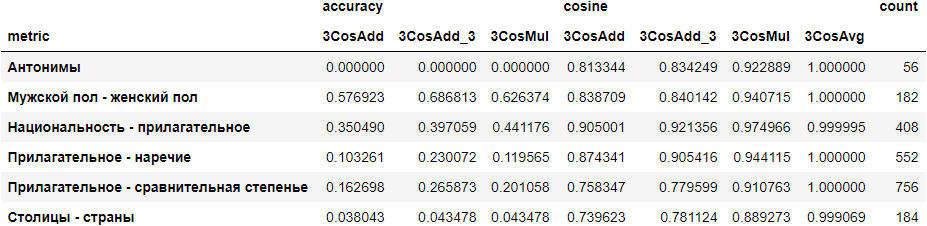
\includegraphics[width=0.9\linewidth]{image/res_DeepPavlov-liter_3 }
	\caption*{Рис. Г9. Результаты тестирования для модели DeepPavlov-liter\_3 }
	\label{fig:resDeepPavlov-liter3 }
\end{figure}

\begin{figure}[H]
	\centering
	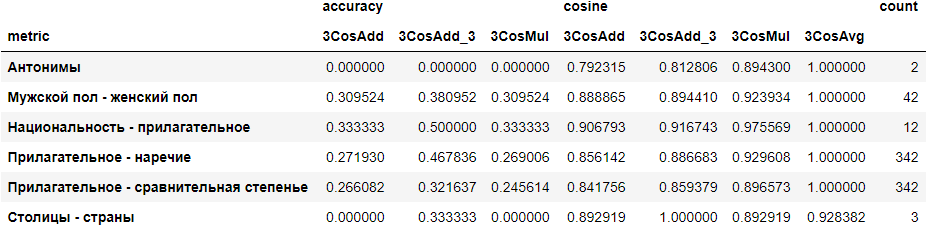
\includegraphics[width=0.9\linewidth]{image/res_DeepPavlov-polit }
	\caption*{Рис. Г10. Результаты тестирования для модели DeepPavlov-polit }
	\label{fig:resDeepPavlov-polit }
\end{figure}

\begin{figure}[H]
	\centering
	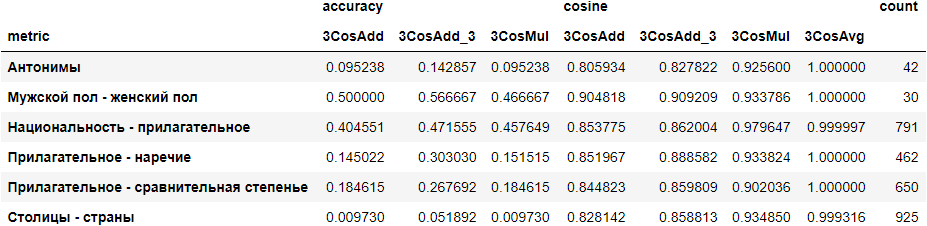
\includegraphics[width=0.9\linewidth]{image/res_DeepPavlov-polit_2 }
	\caption*{Рис. Г11. Результаты тестирования для модели DeepPavlov-polit\_2 }
	\label{fig:resDeepPavlov-polit2 }
\end{figure}

\begin{figure}[H]
	\centering
	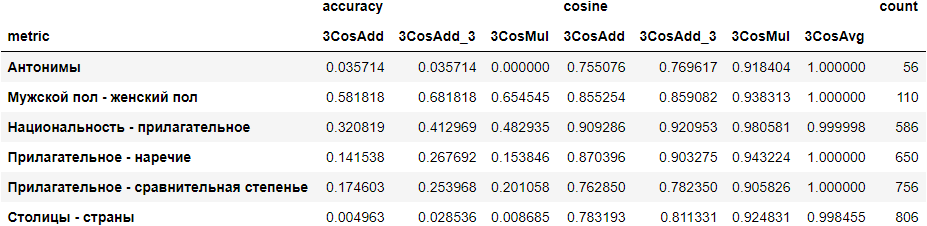
\includegraphics[width=0.9\linewidth]{image/res_DeepPavlov-polit_3 }
	\caption*{Рис. Г12. Результаты тестирования для модели DeepPavlov-polit\_3 }
	\label{fig:resDeepPavlov-polit3 }
\end{figure}

\begin{figure}[H]
	\centering
	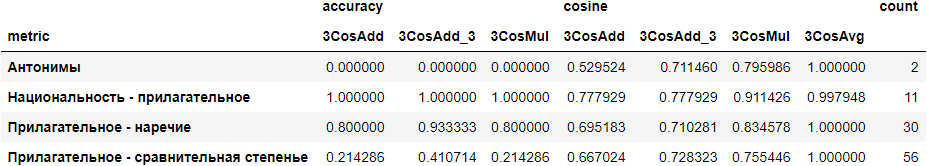
\includegraphics[width=0.9\linewidth]{image/res_elmo-DeepPavlov-liter }
	\caption*{Рис. Г13. Результаты тестирования для модели elmo-DeepPavlov-liter }
	\label{fig:reselmo-DeepPavlov-liter }
\end{figure}

\begin{figure}[H]
	\centering
	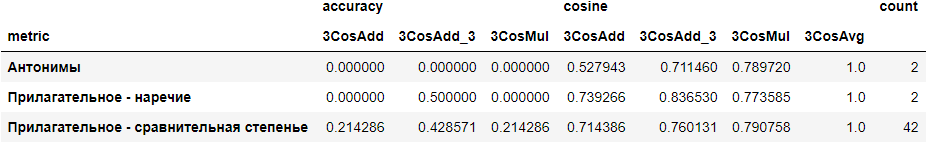
\includegraphics[width=0.9\linewidth]{image/res_elmo-DeepPavlov-polit }
	\caption*{Рис. Г14. Результаты тестирования для модели elmo-DeepPavlov-polit }
	\label{fig:reselmo-DeepPavlov-polit }
\end{figure}


\end{document}